%!TEX root = ../Main.tex
%\eject

\begin{figure*}[ht!]
\begin{center}
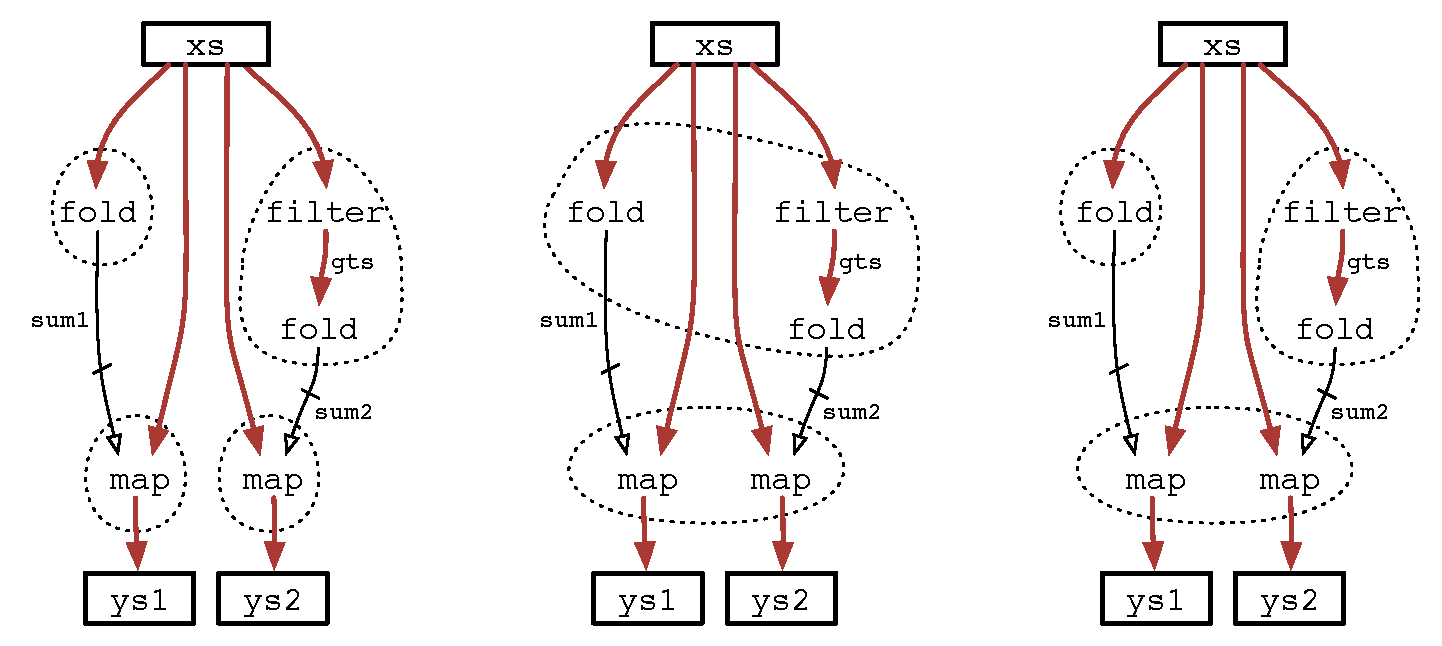
\includegraphics[scale=0.5]{figures/ex1-compare.pdf}
\end{center}

\caption{Clusterings for normalize2 example: with stream fusion; our system; best imperative system}
\label{f:normalize2-cluterings}
\end{figure*}


\section{Combinator normal form}
We can accept functions written in \emph{combinator normal form}, which is a specialised form of first-order array programs detailed in Figure~\ref{f:CombinatorNormalForm}.
This form is a list of combinator bindings, where variables are split into scalar and array variables.
The main restriction is that worker functions may only reference scalar variables, nor may they include any array combinators.

We support the following combinators: $@map@_n$, @filter@, @fold@, @gather@ and @cross@.
Most of these are standard combinators except for @gather@ and @cross@, however $@map@_n$ differs slightly from usual @map@ in that it takes $n$ arrays of the same length, and applies the worker function to all elements of the same index.
The @gather@ combinator is equivalent to @gather xs ys = map (index xs) ys@.
However, as we support no @index@ operation, and worker functions may not refer to arrays, @gather@ is implemented as a primitive.
The @cross@ combinator takes two arrays, and returns the cartesian product of the two.

Since it is unlikely that an entire function will be comprised of these few combinators, we support one additional binding type: @external@.
This signifies that the referenced variables are used by a computation that is not a primitive combinator, and must be materialised fully in memory at this stage.
The @external@ also lists the variables produced by the external computation.
Without knowing the nature of the computation expressed by @external@, we must naturally take a conservative view, and allow no fusion to occur between at these points. They are, in effect, fusion barriers, forcing arrays and scalars to be fully computed before continuing.
This also allows us to support combinators other than those here, but as they must be treated conservatively will likely be less optimal than if they were implemented as primitives.

It is important to note that because of the purity of Haskell, we are free to take certain liberties when fusing the program.
None of the worker functions, nor any @external@ computations may produce visible side-effects; the only observable effect must be to produce their output.
This means that any reordering of the program is allowed, as long as mentioned variables are bound beforehand.
%!TEX root = ../Main.tex
\begin{figure}
\begin{tabbing}
MMMM        \= MM \= MMMMMMMMM \= \kill
$scalar$    \> $\to$ \> (scalar variable) \\
$array$     \> $\to$ \> (array variable)  \\
$f$         \> $\to$ \> (worker function) \\
$fun$       \> $\to$ \> $f~scalar\ldots$
\\[2ex]
$bind$      \> @::=@ \> $scalar$ \> $=~sbind$ \\
            \> $~|$  \> $array$  \> $=~abind$ \\
            \> $~|$  \> $scalar\ldots,array\ldots$ \> $=~@external@~scalar\ldots~array\ldots$
\end{tabbing}

\begin{tabbing}
MMMM        \= MM \= MMMMM \= MMMMMM \= M \= MMMM \= MMMMMM \= \kill
$sbind$     \> @::=@ \> $@fold@$     \> $fun~~ array$
\\[1ex]

$abind$     \> @::=@ \> $@map@_n$    \> $fun~~ array^n$ 
            \> $~|$  \> $@filter@$   \> $fun~~ array$   \\
            \> $~|$  \> $@generate@$ \> $scalar~~ fun$  
            \> $~|$  \> $@gather@$   \> $array~~ array$ \\
            \> $~|$  \> $@cross@$    \> $array~~ array$
\\[1ex]
$function$  \> @::=@ \> $\lambda scalar\ldots~array\ldots~\to$ \\
            \>          \> $@let@~bind\ldots$                  \\
            \>          \> $@in@~(scalar\ldots,~array\ldots)$
\\[3ex]
$@fold@$     \> $:~ (a \to a \to a) \to @Array@~~ a \to a$     \\
$@map@_n$    \> $:~ (\{a_i          \to\}^{\;i\; \gets 1 \dots n}~~ b)  \to
                       \{@Array@~~ a_i \to\}^{\;i\; \gets 1 \dots n}~~ @Array@~~ b$ \\
$@filter@$   \> $:~ (a \to @Bool@) \to @Array@~~ a \to @Array@~~ a$      \\
$@generate@$ \> ~~ $:~ @Nat@ \to (@Nat@ \to a) \to @Array@~~ a$          \\
$@gather@$   \> ~~ $:~ @Array@~~ a \to @Array@~~ @Nat@  \to @Array@~~ a$ \\
$@cross@$    \> ~~ $:~ @Array@~~ a \to @Array@~~ a ~~~~ \to @Array@~~ a$
\end{tabbing}
\caption{Combinator normal form}
\label{f:CombinatorNormalForm}
\end{figure}




